\documentclass[tikz,border=4pt]{standalone}
% Estilos compartilhados pelos diagramas dos estágios e módulos do Core.
\usetikzlibrary{arrows.meta, positioning, calc, shapes.geometric, fit}

\tikzset{
  >={Stealth[length=2.2mm]},
  bloco/.style={draw, rounded corners=2pt, minimum width=24mm, minimum height=9mm,
                align=center, font=\small, fill=blue!6},
  regpipe/.style={draw, minimum width=9mm, minimum height=48mm, align=center,
                  font=\small, fill=gray!25},
  mux/.style={draw, trapezium, trapezium angle=70, shape border rotate=90,
              minimum height=11mm, minimum width=7mm, inner sep=1pt, align=center,
              font=\scriptsize, fill=orange!15},
  ctrl/.style={draw, rounded corners=2pt, minimum width=24mm, minimum height=9mm,
               align=center, font=\small, fill=green!10},
  opcional/.style={bloco, dashed, fill=yellow!12},
  externo/.style={draw, rounded corners=2pt, minimum width=24mm, minimum height=9mm,
                  align=center, font=\small, fill=red!8},
  dado/.style={->, thick},
  sinal/.style={->, dashed},
  rotulo/.style={font=\scriptsize, midway, above, inner sep=1pt},
  titulo/.style={font=\bfseries\normalsize}
}

\begin{document}
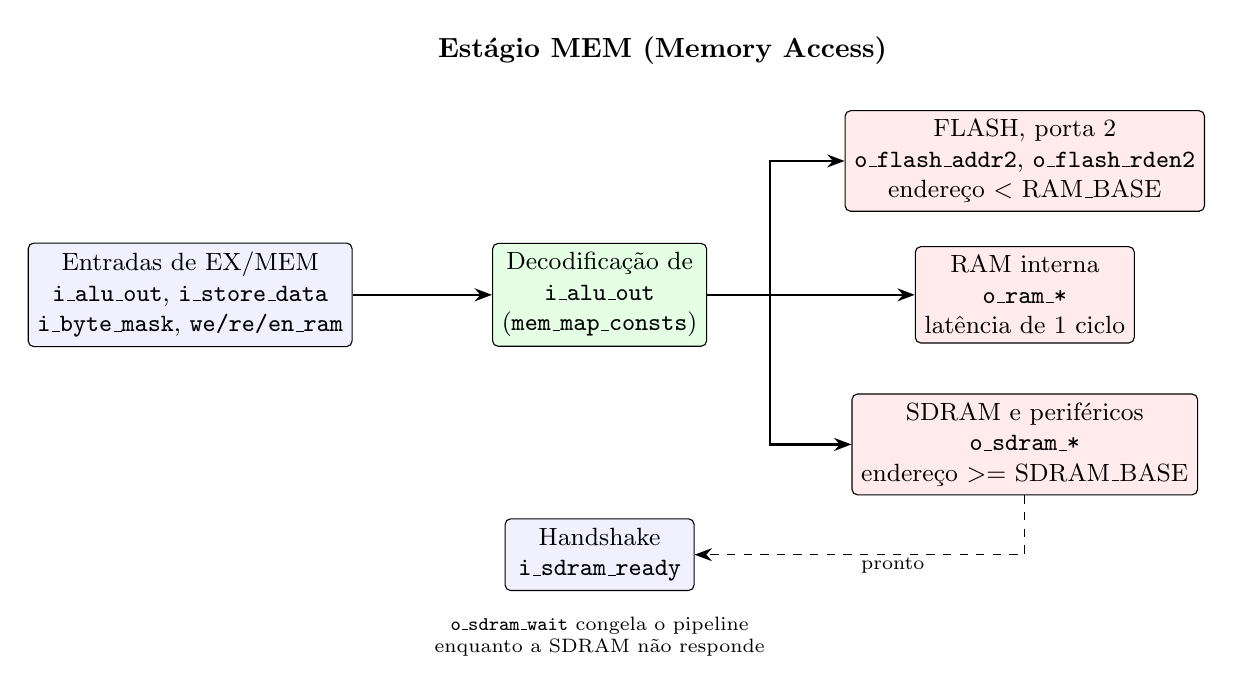
\begin{tikzpicture}
  \node[titulo] at (6,4.6) {Estágio MEM (Memory Access)};
  \node[bloco] (in) at (0,1.5) {Entradas de EX/MEM\\\texttt{i\_alu\_out}, \texttt{i\_store\_data}\\\texttt{i\_byte\_mask}, \texttt{we/re/en\_ram}};
  \node[ctrl] (dec) at (5.2,1.5) {Decodificação de\\\texttt{i\_alu\_out}\\(\texttt{mem\_map\_consts})};
  \node[externo] (fl) at (10.6,3.2) {FLASH, porta 2\\\texttt{o\_flash\_addr2}, \texttt{o\_flash\_rden2}\\endereço \textless{} RAM\_BASE};
  \node[externo] (ram) at (10.6,1.5) {RAM interna\\\texttt{o\_ram\_*}\\latência de 1 ciclo};
  \node[externo] (sd) at (10.6,-0.4) {SDRAM e periféricos\\\texttt{o\_sdram\_*}\\endereço \textgreater= SDRAM\_BASE};
  \node[bloco] (rdy) at (5.2,-1.8) {Handshake\\\texttt{i\_sdram\_ready}};

  \draw[dado] (in) -- (dec);
  \draw[dado] (dec.east) -- ++(0.8,0) |- (fl.west);
  \draw[dado] (dec) -- (ram);
  \draw[dado] (dec.east) -- ++(0.8,0) |- (sd.west);
  \draw[sinal] (sd.south) |- node[rotulo, pos=.7, below] {pronto} (rdy.east);
  \node[font=\scriptsize, below=2mm of rdy, align=center] {\texttt{o\_sdram\_wait} congela o pipeline\\enquanto a SDRAM não responde};
\end{tikzpicture}
\end{document}
